\pagebreak

\section{Datatypes}

Für die interne Datenhaltung und -verwaltung werden Klassen in der
Package \lstinline{datatypes} zur Verfügung gestellt. Sämtliche
interne Datentypen wie Boolean, Zahlen, Strings, Tupel, Tabellen
und Objekte erben von \lstinline{InternalObject}. So kann jede Variable, die
in Tabulang erstellt wird, annotiert und diese Annotationen durch
Aufbau einer Baumstruktur von Eltern-Objekten geerbt werden.

In diesem Kapitel wird die Umsetzung der internen Datentypen erläutert
sowie einige Fehlerbehandlungen aufgegriffen. Das Klassendiagramm in 
Abbildung \ref{fig:datatypes-uml} soll hierzu eine Übersicht über die
Zusammenhänge und die zur Verfügung gestellten Methoden geben. Zu Zwecken
der Übersicht wurden auf einige Methoden wie Getters und Setters verzichtet.

\begin{figure}[]
\centering
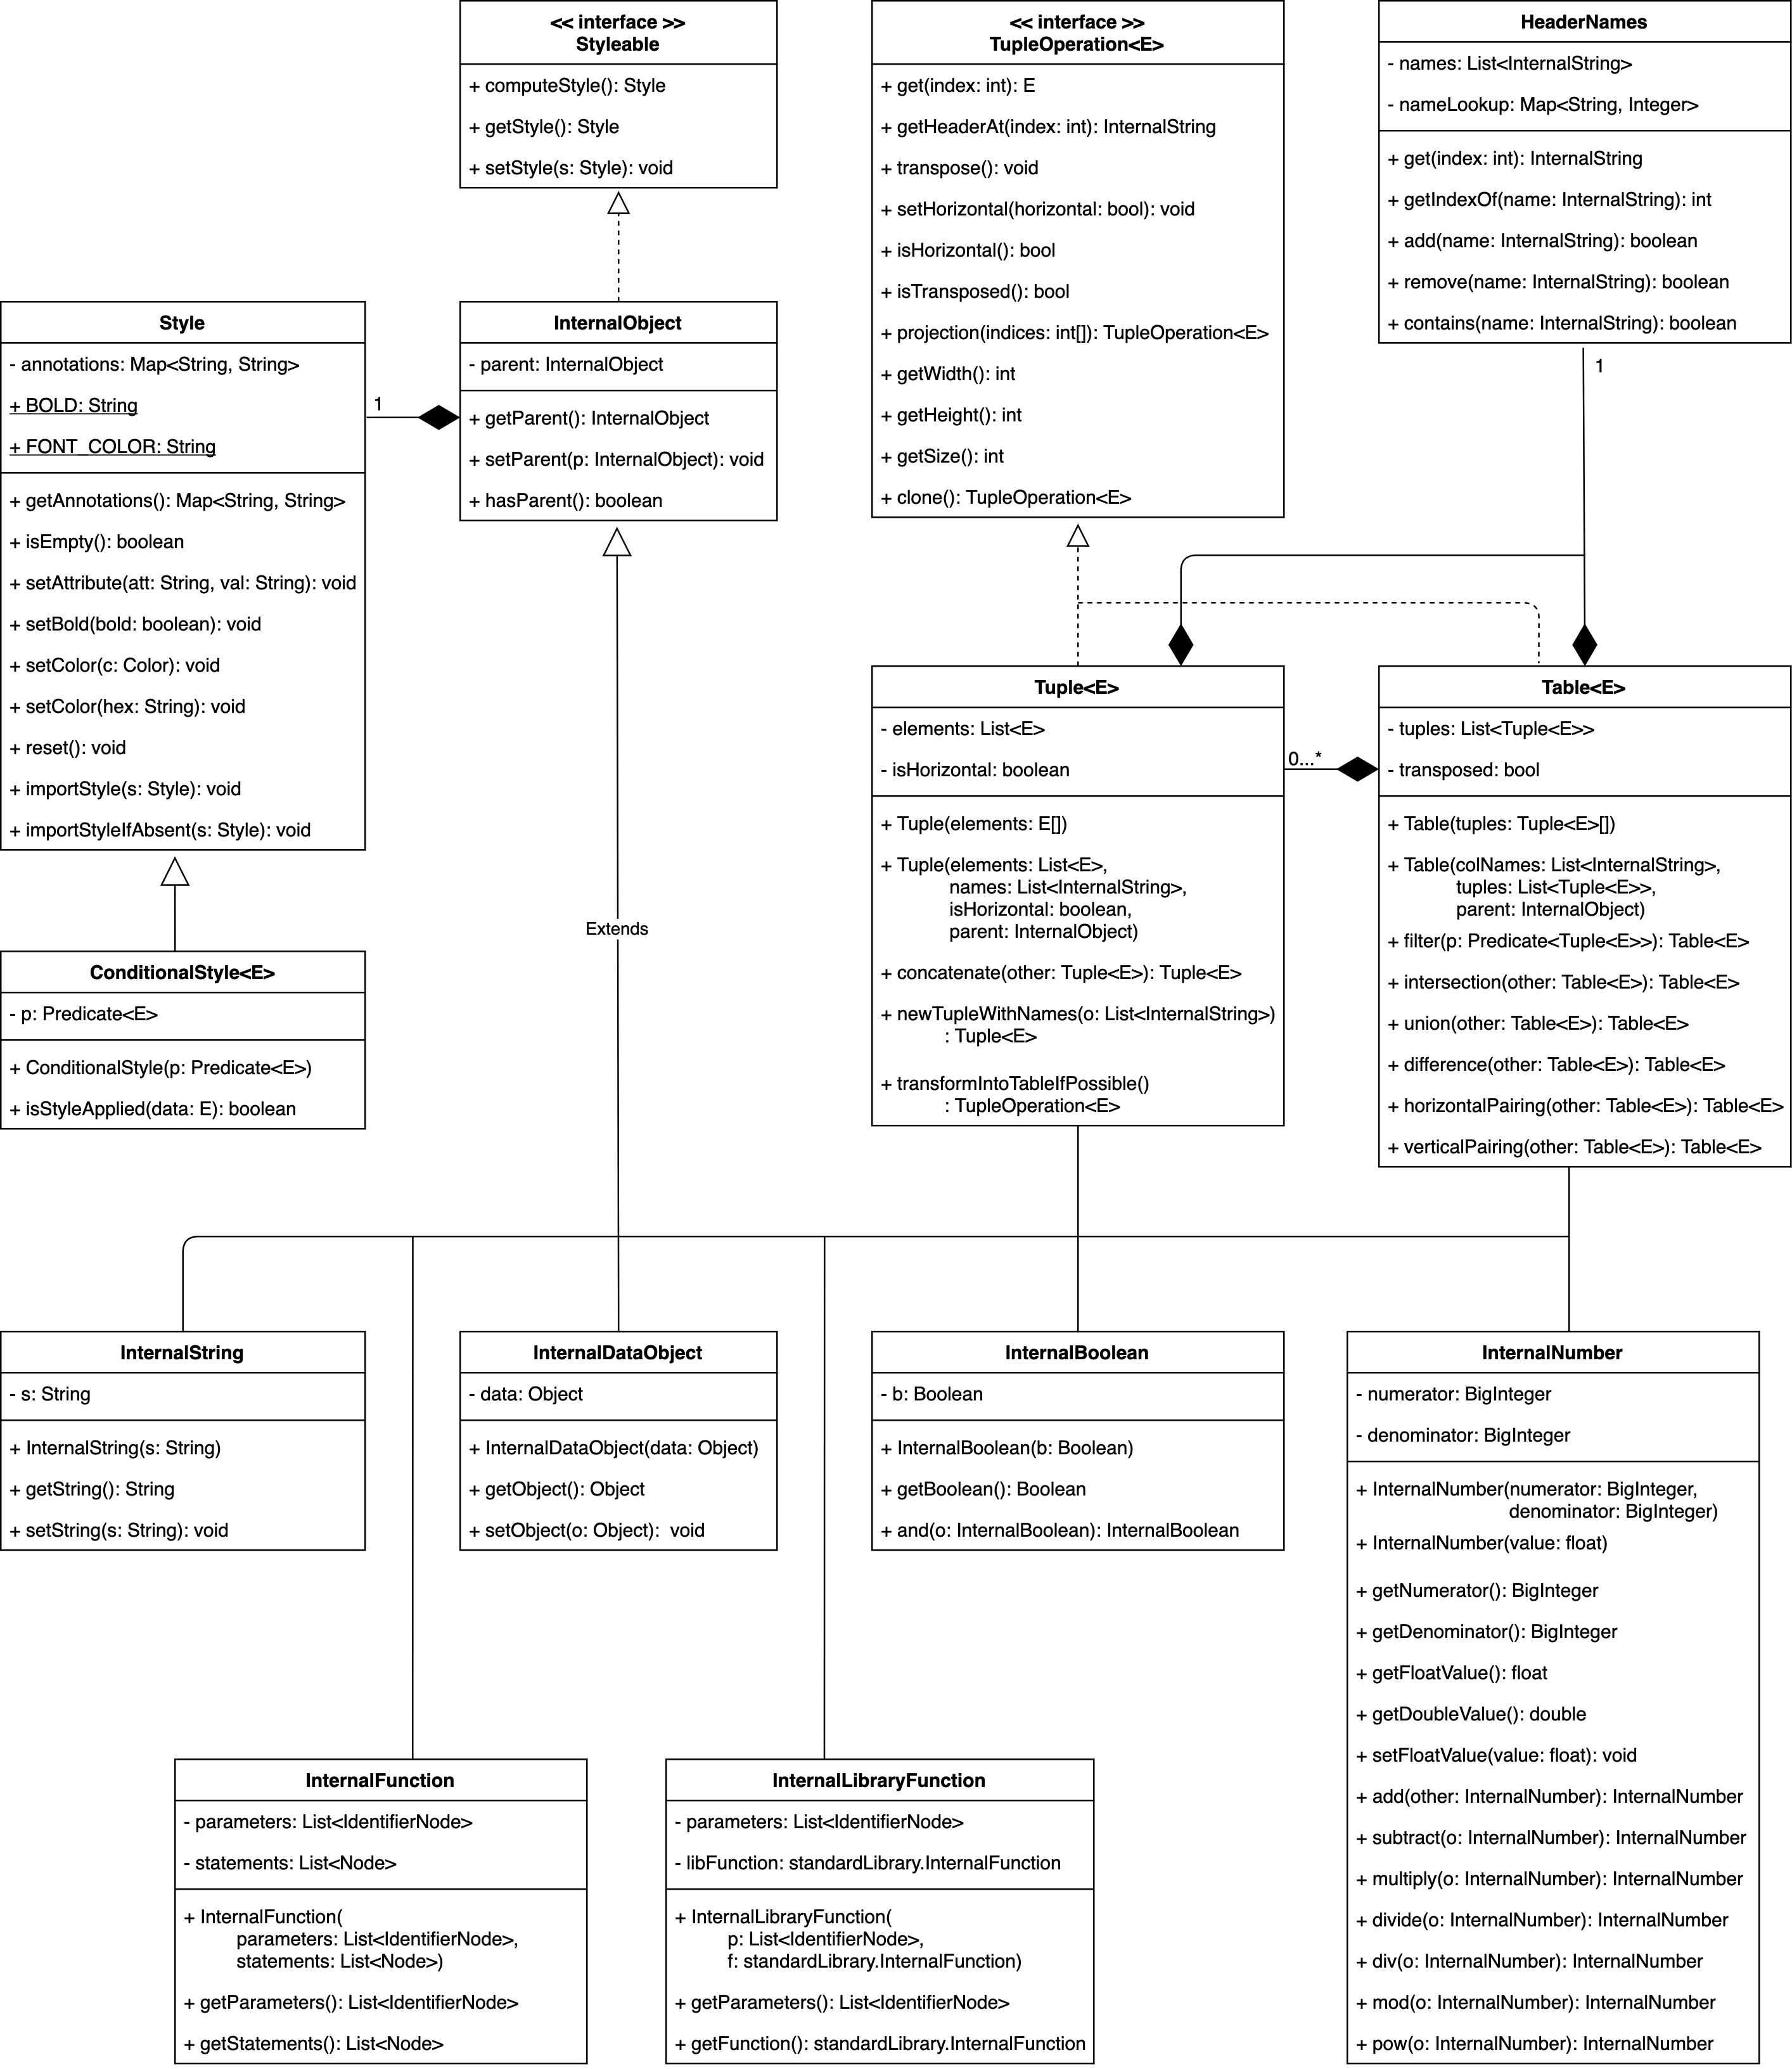
\includegraphics[width=\textwidth]{images/datatypes-uml.png}
\caption{Klassendiagramm - Datentypen}
\end{figure}\label{fig:datatypes-uml}

\subsection{Objects und Styles}

Jedes erzeugbare Objekt in Tabulang wird
in eine interne Datenhaltungsklasse gepackt,
welches die Anforderung erfüllt, alle Variable annotierbar zu machen.

Eine Annotation ist nichts anderes als ein
String-Key-Value-Paar das in einer \lstinline{map} gespeichert wird.
Mit jeder Erzeugung eines Objektes in Tabulang
wird der Variable solch eine Map angehängt, der beispielsweise
% Die zwei Leerzeichen nach dem 'bold' sind Absicht, bidde so lassen, dange
mit \lstinline{mark 'bold'  as 'true'} eine Annotation beigefügt
werden kann.

Annotationen sind vererbbar. Interne Objekte, die in Containern
enthalten sind, erben deren Annotationen, sofern bei der Vererbung keine
bereits vorhandenen Annotationen überschrieben werden.

Das Interface \lstinline{Styleable} bietet dazu lediglich die zu
implementierenden Methoden, die Klasse \lstinline{InternalObject}
die eigentliche Umsetzung. Die eigentlichen Annotationen werden in
\lstinline{Style}-Objekte gepackt.

Nachdem \lstinline{Styleable} und \lstinline{Style} recht eng miteinander
gekoppelt sind, war eine Überlegung, die Klasse \lstinline{Style}
mit den entsprechenden Methoden aus \lstinline{Styleable} abstrakt zu
machen um sich das Interface zu sparen. Es wurde sich aber aus zwei
konzeptionellen Gründen dagegen entschieden. Erstens sind Styles oder Annotationen
etwas, das Objekte \textit{besitzen} und nicht erben. Zweitens
können in Java mittels \lstinline{extends} von maximal einer Klasse geerbt
werden. Mit der Generalisierung durch einem Interface ist somit
mehr Flexibilität geboten.

\lstinline{InternalObject} bildet nun die Umsetzung der drei Methoden
\lstinline{computeStyle}, \lstinline{getStyle} und \lstinline{setStyle}.
Zusätzlich besitzt die Klasse ein \lstinline{parent} Attribut des gleichen
Typs, wodurch eine Baumstruktur von internen Objekten erzeugt werden kann.

In der Baumstruktur liegt der Hauptunterschied zwischen den Methoden \lstinline{computeStyle}
und \lstinline{getStyle}. Bei \lstinline{getStyle} wird selbsterklärend das gesetzte
\lstinline{Style}-Objekt in der Klasse zurückgegeben. In \lstinline{computeStyle}
wird ein neues \lstinline{Style}-Objekt erzeugt, dessen Annotations-Map durch das
rekursive durchhangeln durch die Elternobjekte befüllt wird. Hierbei werden nur
solche Annotationen hinzugefügt, die sich nicht bereits in der Map befinden (siehe
\lstinline{importStyleIfAbsent} in der \lstinline{Style} Klasse).\\

Die \textbf{Konstanten} in \lstinline{Style} wie zum Beispiel \lstinline{BOLD},
\lstinline{FONT_FAMILY} oder \lstinline{BACKGROUND_COLOR} werden im Wesentlichen
zum Import und Export von ods-Dateien benötigt, worauf in Kapitel \ref{subsectionLibreOffice}
eingegangen wird.

\lstinline{Style} bietet neben der Standard \lstinline{setAttribute} Methode
eine Reihe an Settern, mit der diese Konstanten gesetzt werden können. Wie sich
später aber herausstellte waren diese bis jetzt nicht sonderlich hilfreich, zumal es für
den Interpreter keine Tabulang-spezifische Konstrukte gibt, die von dem Aufruf
der Setter-Methoden profitieren könnten.

Nichtsdestotrotz wird in Listing \ref{lst:stylesetter} beispielhaft gezeigt, wie bei einem zukünftigen
Tabulang-Team diese Methoden zur Geltung kommen könnten.

\begin{lstlisting}[caption={Attribute in der Style-Klasse setzen}, label={lst:stylesetter}, language=Java]
// Diese drei Methodenaufrufe sind äquivalent
s.setStyle(Style.FONT_COLOR, "#00FF10");
s.setColor("#00FF10");
s.setColor(new Color(0, 255, 16));
\end{lstlisting}

Zu guter Letzt gab es noch die Idee, \textbf{konditionelle Styles} mittels
\lstinline{ConditionalStyle} einzuführen. Wenn in Tabulang
beispielsweise eine Variable mit \lstinline{mark 'bold'  as 'true'  if mapvalue > 0} annotiert
wird, sollte mit jedem \lstinline{computeStyle} Aufruf festgelegt werden, ob mit
dem aktuellen Wert in der Variable der Style tatsächlich gesetzt wird oder nicht.

Die genaue Umsetzung erwies sich jedoch als etwas komplizierter als erwartet. Um
eine Abfrage mittels des Predicate durchführen zu können, muss in \lstinline{computeStyle}
der aktuelle Wert bekannt sein. \lstinline{InternalObject} hat allerdings kein
Attribut, das den Wert der Variablen speichert - hierfür sind die Kindklassen vorgesehen.
Zudem ist noch nicht gewiss, wie mehrere Styles mit unterschiedlichen Konditionen innerhalb
einer Variablen gehandhabt werden sollten.

Folgende Lösungsansätze könnten in Betracht gezogen werden, die eine wesentliche Umstruktierung
der internen Datenhaltung erfordert und aus zeitlichen Gründen nicht mehr umgesetzt werden konnte.

\begin{itemize}
    \item Eine abstrakte Getter-Funktion in \lstinline{InternalObject}, die den aktuellen Wert der Variablen zurückgibt.
    \item Ein generisches Daten-Attribut in \lstinline{InternalObject}, das von den Kindklassen immer auf dem aktuellsten Stand gehalten wird.
    \item Anstelle eines Predicates werden in \lstinline{ConditionalStyle} Nodes gespeichert, die der Interpreter auswerten kann.
\end{itemize}

\subsection{Numbers}

\subsection{Tuples}

Ein Tupel ist eine geordnete Menge an Elementen, die von \lstinline{InternalObject} erben.
Tupel sind typisiert: jedem Element im Tupel wird ein String-Wert zugewiesen werden, über dem
das Element referenziert werden kann.

Die Typisierung wird über \lstinline{HeaderNames} realisiert. Das Ziel ist, den Index
eines Elements in nahezu konstanter Laufzeit zu ermitteln. Dafür spielen die zwei Attribute
\lstinline{names} (eine Liste) und \lstinline{nameLookup} (eine HashMap) in Tandem zusammen.
In \lstinline{names} wird die geordnete Menge an Strings gespeichert, in \lstinline{nameLookup}
die aktuellen Indizes der Strings.

In der Sprache kann ein Element auf zwei Arten referenziert werden, entweder über dessen typisierten Strings oder
über den Index (siehe Listing \ref{lst:tuplerefs}). Die Referenzierung wird vom Parser als \lstinline{InternalString}
übergeben. Über den Methodenaufruf \lstinline{getIndexOf(internalString)} in \lstinline{HeaderNames}
werden folgende Fälle abgearbeitet.

\begin{enumerate}
    \item Befindet sich \lstinline{internalString} in \lstinline{nameLookup}, so gebe den zugehörigen Indexwert zurück.
    \item Befindet sich \lstinline{internalString} nicht in \lstinline{nameLookup}, versuche den String in eine Zahl zu konvertieren.
    \begin{enumerate}
        \item Lässt sich \lstinline{internalString} in eine Zahl $x$ konvertieren und liegt die Zahl innerhalb des Wertebereichs $0 \leq x < \textrm{getSize()}$, gib die Zahl zurück.
        \item Sonst werfe eine \lstinline{TupleNameNotFoundException}.
    \end{enumerate}
\end{enumerate}

Namen dürfen in der Typisierung nicht doppelt erscheinen. In solchen Fällen wird eine \lstinline{DuplicateNamesException} geworfen.

Zudem sollte bei der Zuweisung einer Typisierung dieselbe Anzahl an Strings übergeben werden, die im Tupel vorhanden sind. Ansonsten
wird eine \lstinline{ArrayLengthMismatchException} geworfen.

\begin{lstlisting}[caption={Referenzierung von Tupelelementen in Tabulang}, label={lst:tuplerefs}, language=Java]
s := ['Hans', 'Peter', 67];
setHeaderNames(s, ['Vorname', 'Nachname', 'Alter']);

// beides gibt 'Peter' zurück
s.'Nachname';
s.'1';
// wirft eine TupleNameNotFoundException
s.'3';
// wirft eine DuplicateNamesException
setHeaderNames(s, ['Name', 'Name', 'Alter']);
// wirft eine ArrayLengthMismatchException
setHeaderNames(s, ['Vorname', 'Nachname', 'Alter', 'Wohnort']);
\end{lstlisting}

Ein Tupel besitzt neben den Elementen und deren Typisierung auch eine Orientierung. Diese kann auf \lstinline{horizontal} (Standard)
oder \lstinline{vertical} gesetzt werden, wie in Listing \ref{lst:tupleprint} zu sehen ist.
Die \lstinline{toString} Methode in \lstinline{Tuple} sorgt dafür, dass
je nach gegebener Ausrichtung des Tupels die Elemente gut lesbar sind.

\begin{lstlisting}[caption={Tupelausgabe mit gegebener Orientierung}, label={lst:tupleprint}, language=Java]
print(horizontal s);
// Vorname | Nachname | Alter
// Hans    | Peter    | 67
print(vertical s);
// Vorname  | Hans
// Nachname | Peter
// Alter    | 67
\end{lstlisting}

Diverse Operationen, die auf einem Tupel in der Tabulang Sprache ausgeführt werden können, sind auf die jeweiligen
Methoden in der Klasse implementiert. Der Hauptfokus lag unter Anderem darin, das Konzept einer funktionalen Programmiersprache
beizubehalten: das Tupelobjekt wird beim Aufruf einer solchen Methode nicht verändert und gibt stattdessen ein neues Objekt zurück.

In der folgenden Tabelle seien die Operationen kurz angeführt. Nachdem diese in der Sprachbeschreibung detailliert beschrieben sind, wird hier
nicht näher darauf eingegangen.

\begin{center}
    \begin{tabular}{ |l|l| } 
        \hline
        Operation & Klassenmethode \\ 
        \hline
        Änderung der Tupelorientierung & \texttt{setHorizontal(boolean horizontal)}* \\ 
        Konkatenation & \texttt{concatenate(Tuple<E> other)} \\
        Projektion & \texttt{projection(InternalString... names)} \\
        Re-Typisierung & \texttt{newTupleWithNames(List<InternalString> newNames)} \\
        \hline
    \end{tabular}
\end{center}

*Hier wird kein neues Tupelobjekt erzeugt. Stattdessen sollte \lstinline{clone()} verwendet werden und auf das geklonte Tupel die Orientierung gesetzt werden.

Exceptions, die bei diesen Operationen geworfen werden können, ähneln sich der in Listing \ref{lst:tuplerefs}. Werden
beispielsweise zwei Tupel konkateniert, die die gleiche Typisierung besitzen, wird eine \lstinline{DuplicateNamesException} geworfen.
Wird bei der Projektion ein Name nicht gefunden, wird eine \lstinline{TupleNameNotFoundException} geworfen. Bei der Re-Typisierung
könnte eine\\
\lstinline{ArrayLengthMismatchException} geworfen werden.

Letzteres bieten sowohl \lstinline{Tuple} als auch \lstinline{HeaderNames} eine Konkretisierung der Methode\\
\lstinline{iterator()}, womit
das Iterieren durch alle Elemente mittels einer for-each-Schleife möglich ist.

\subsection{Tables}

Tabellen sind im Wesentlichen Tupel, die wiederum Tupel mit jeweils gleich vielen Elementen besitzen.
Somit ähneln sich Tupel und Tabellen in ihrer Funktionsweise, weshalb die Einführung eines \lstinline{TupleOperation} Interface für sinnvoll betrachtet wurde.

Für Verwirrung könnte hier nur die Orientierung sorgen. In Tupeln spricht man davon, ob diese horizontal oder vertikal sind.
Tabellen dagegen können transponiert oder nicht transponiert sein. Wenn standardmäßig horizontale Tupel erzeugt und in eine Tabelle
gepackt werden, ist diese nicht transponiert. Wird eine Tabelle transponiert, so wird die Orientierung aller darin enthaltenen Tupel
auf vertikal gesetzt.

Nach dem selben funktionalen Schema wie bei Tupel wird mit jeder Operation auf einer Tabelle mit Ausnahme der Transponierung
ein neues Tabellenobjekt erzeugt. Auch wenn das vielleicht der sicherste Weg ist, nimmt man doch deutliche Einbußen in Leistung
und Speicherplatz hin. Für solche Zwecke wurden unter den Tests auch Benchmarks in \texttt{test/benchmarks} eingeführt, die jedoch
noch nicht sinnvoll eingesetzt werden konnten.

Im Folgenden seien die Tabellenoperationen zusammen mit ihren korrespondierenden Klassenmethoden kurz aufgeführt.
Für die detaillierte Funktionsweise wird wieder auf die Sprachbeschreibung bzw. die Dokumentation der Bibliothek gewiesen.

\begin{center}
    \begin{tabular}{ |l|l| } 
        \hline
        Operation & Klassenmethode \\ 
        \hline
        Transponierung & \texttt{transpose()}* \\ 
        Filter & \texttt{filter(Predicate<Tuple<E> > p)} \\
        Projektion & \texttt{projection(InternalString... names)} \\
        Schnitt & \texttt{intersection(Table<E> other)} \\
        Vereinigung & \texttt{union(Table<E> other)} \\
        Differenz & \texttt{difference(Table<E> other)} \\
        Horizontale Paarung & \texttt{horizontalPairing(Table<E> other)} \\
        Vertikale Paarung & \texttt{verticalPairing(Table<E> other)} \\
        \hline
    \end{tabular}
\end{center}

*Wie bei Tupel wird beim Transponieren kein neues Objekt erstellt. Stattdessen sollte man \lstinline{clone()} auf das Tabellenobjekt aufrufen und
das geklonte Objekt transponieren.

Die Filter-Methode macht sich Lambda-Funktionen aus Java 8 zunutze. So kann ein Tabellen-Objekt \lstinline{t} nach Tupeln etwa wiefolgt gefiltert werden:\\
\lstinline{t.filter(tuple -> tuple.get(new InternalString("Alter")).getFloatValue() > 18))}.

In \lstinline{intersection} wie auch in \lstinline{union} und \lstinline{difference} wird erwartet, dass beide Tabellen dieselbe Typisierung enthalten.
Ist dies nicht der Fall, wird eine \lstinline{TableHeaderMismatchException} geworfen.\\

Im Allgemeinen bietet die Sprache in Tabulang keine Möglichkeit, Tabellen zu erzeugen.
Stattdessen können Tupel von Tupel erzeugt werden, die sich weiterhin wie Tupel verhalten, bis eine Tabellenoperation darauf
ausgeführt wird. Wird etwa die Filteroperation auf ein Tupel ausgeführt, wird versucht, aus diesem Tupel eine
Tabelle zu erzeugen (siehe hierzu\\
\lstinline{transformIntoTableIfPossible} in der Klasse \lstinline{Tuple}).

Ist die Konvertierung nicht erfolgreich, bleibt das Tupel weiterhin so erhalten. In der Regel wird dann eine \lstinline{IllegalTableArgumentException} geworfen,
da eine Tabellenoperation nicht auf einem Tupel ausgeführt werden kann.

Ein volles Beispiel dazu wird in \ref{lst:tupletotable} gezeigt.

\begin{lstlisting}[caption={Tupel zu Tabellen-Konvertierung}, label={lst:tupletotable}, language=Java]
t := [['Hans','Peter'],['Amelie','Müller'],['Wilhelm','Amerson']];
setHeaderNames(t, ['p1', 'p2', 'p3']);
setHeaderNames(t.'p1', ['Vorname', 'Nachname']);
setHeaderNames(t.'p2', ['Vorname', 'Nachname']);
setHeaderNames(t.'p3', ['Vorname', 'Nachname']);

print(vertical t);
// p1 | Vorname | Nachname\\nHans    | Peter
// p2 | Vorname | Nachname\\nAmelie  | Müller
// p3 | Vorname | Nachname\\nWilhelm | Amerson

filtered := t filter stringLength(Vorname) > 5;
print(filtered);
// Vorname | Nachname
// ------------------
// Amelie  | Müller
// Wilhelm | Amerson
//
// filtered ist nun eine Tabelle
// Variable t bleibt weiterhin ein Tupel
\end{lstlisting}
